

\section{Which detector settings should I choose?}

The choice of the operation settings is very important in order to obtain good quality data. \\
Normally slower settings will reduce the electronics noise and therefore it is possible to work at lower energies, but will saturate for high photon fluxes.\\
On the other hand, faster settings will allow to work with higher photon intensities without pileup, but not to access lower energies because of an higher electronics noise.\\
Therefore it is extremely important to chose adequate settings for the detector depending on the X-ray energy and expected maximum count rate.
In the following is a description of the energy and intensity range coverd by the different settings for each detector.




\subsection{MYTHEN}

Normally the user can follow these rules:
\begin{enumerate}
\item If the X-ray energy is lower than 8~keV the \textit{High gain} setting should be used. Since it is a slow mode of operation it is necessary to take care that the maximum count rate is lower than 100~kcounts/s for all channels (use filters to reduce the beam intensisty).
\item For energies higher than 8~keV, the \textit{Standard} setting is normally fine if the count rate can be kept lower than 300~kcounts/s for all channels (use filters to reduce the beam intensisty). 

\item In case a larger count rate is required in order to keep the acquisition time shorter, the \textit{Fast} setting must be selected. However the maximum count rate should never exceed 1~Mcounts/s   for all channels.
\end{enumerate}


\begin{figure}
\begin{center}
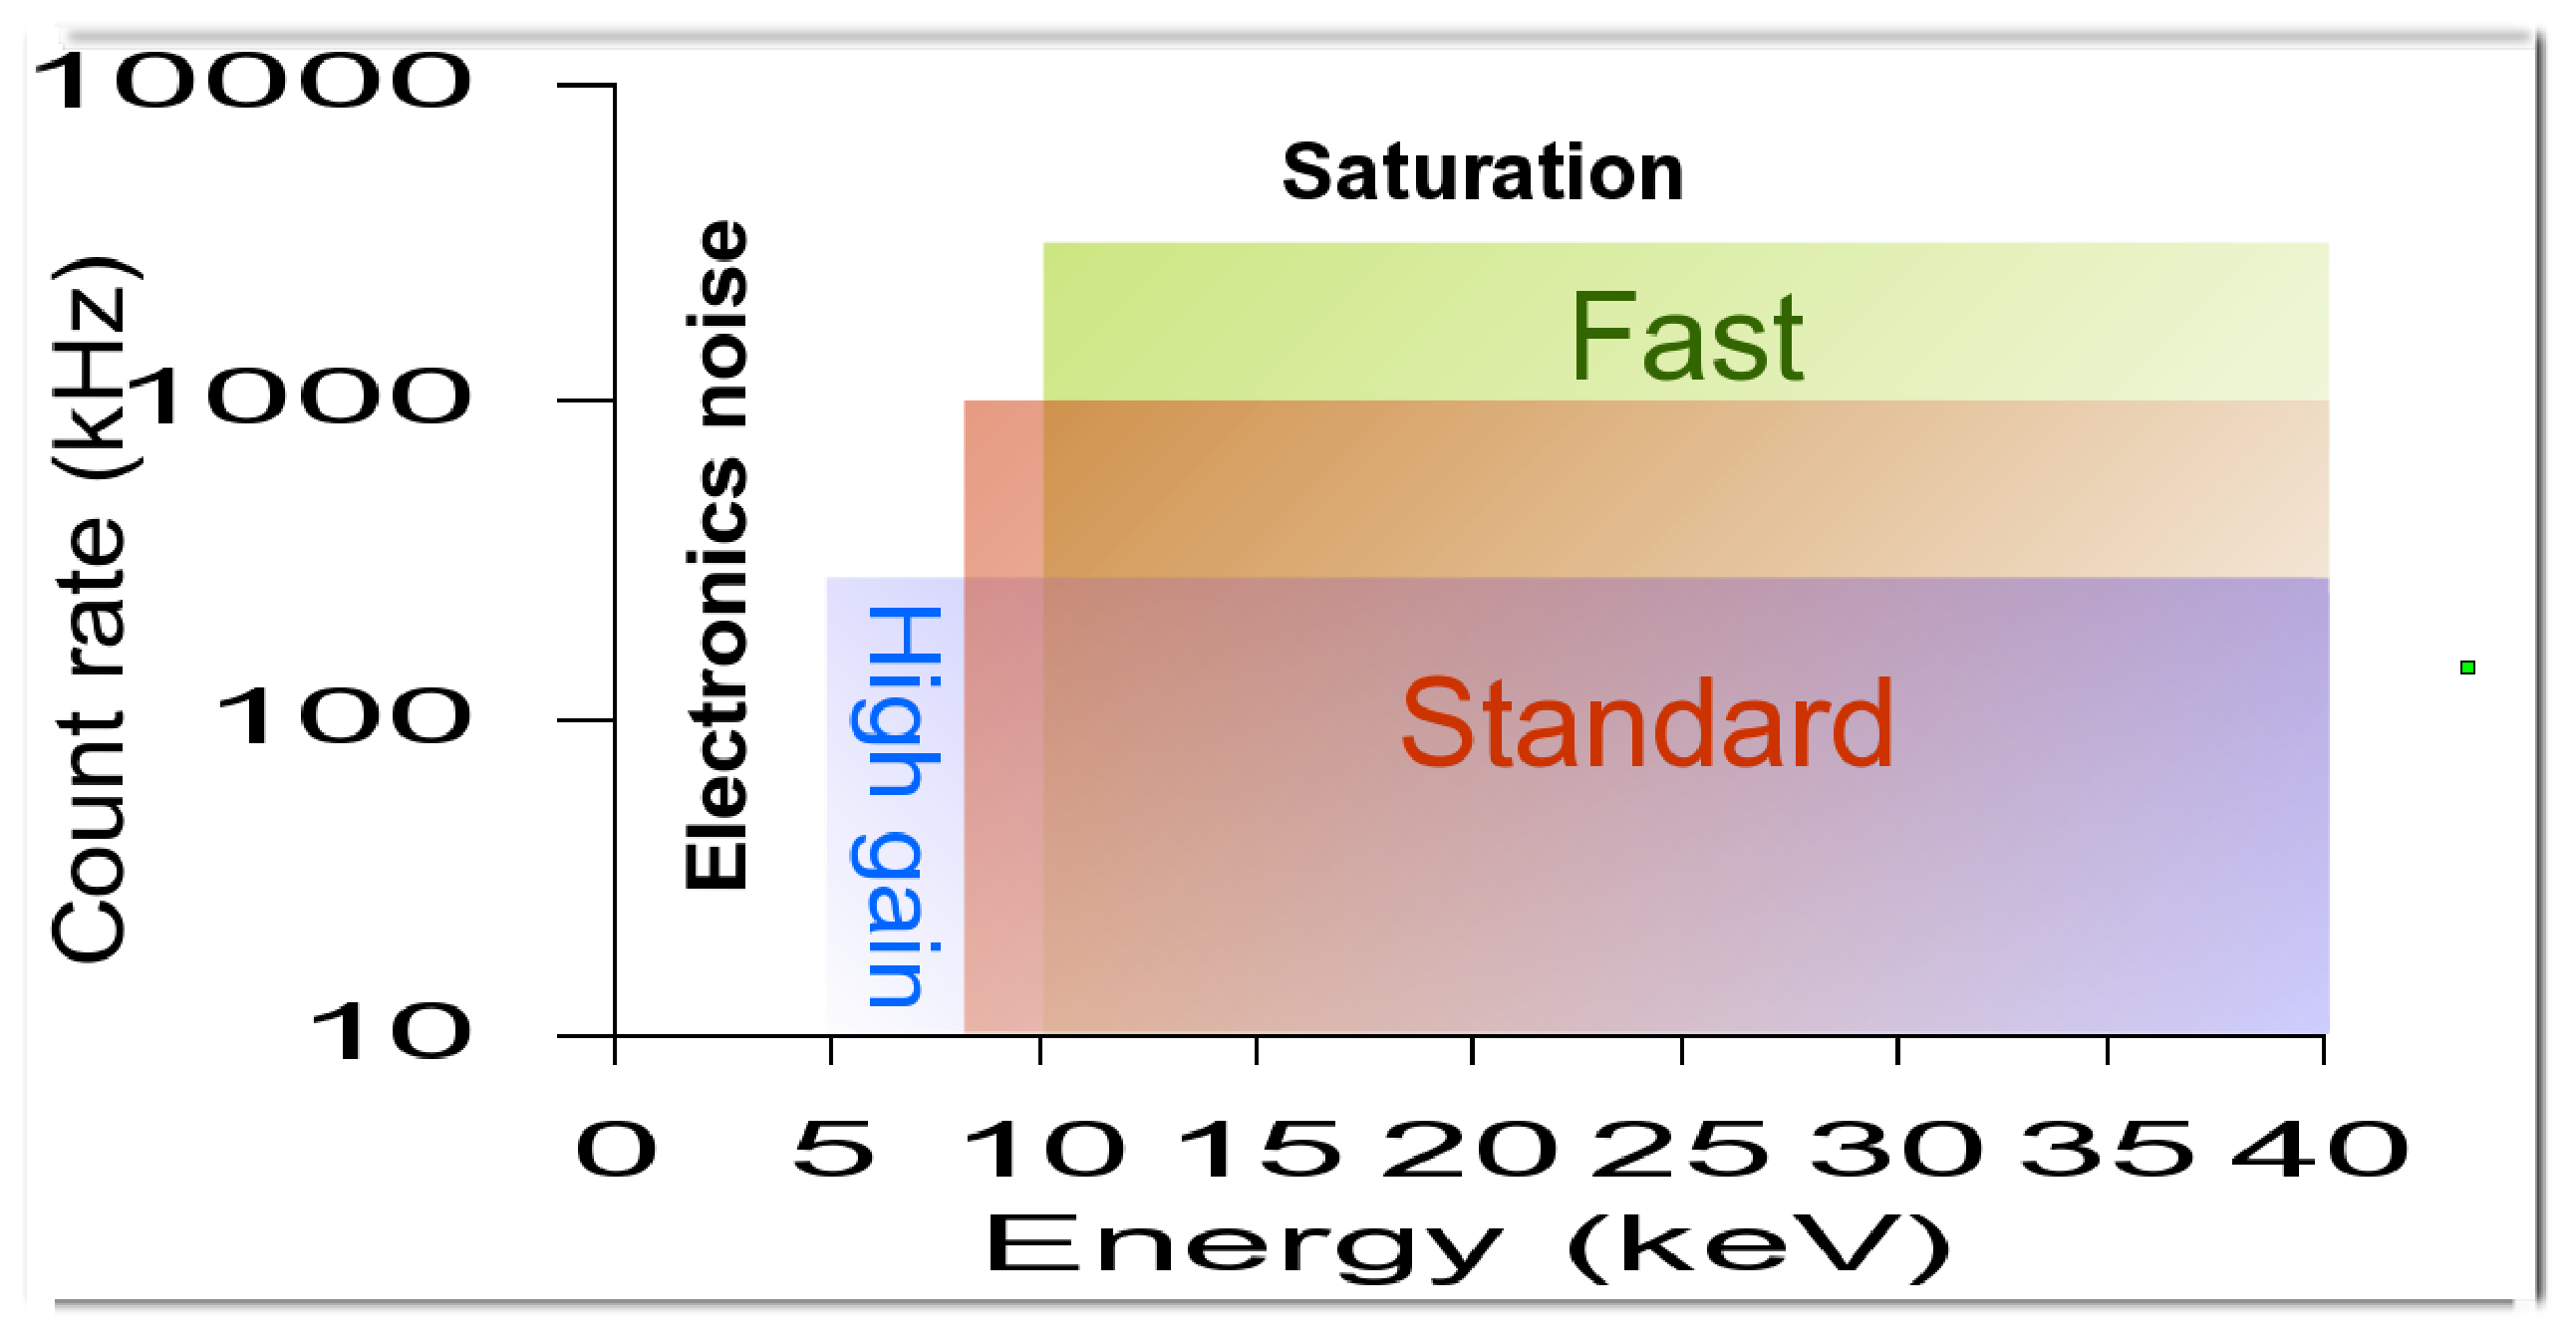
\includegraphics[width=\textwidth]{images/settings}
\end{center}
\caption{Plot indicating the reccomended choice of detector settings as a function of the X-ray energy and maximum count rate per channel..}\label{fig:settings}
\end{figure}


\section{How do I chose the comparator threshold?}

\begin{figure}[b!]
\begin{center}
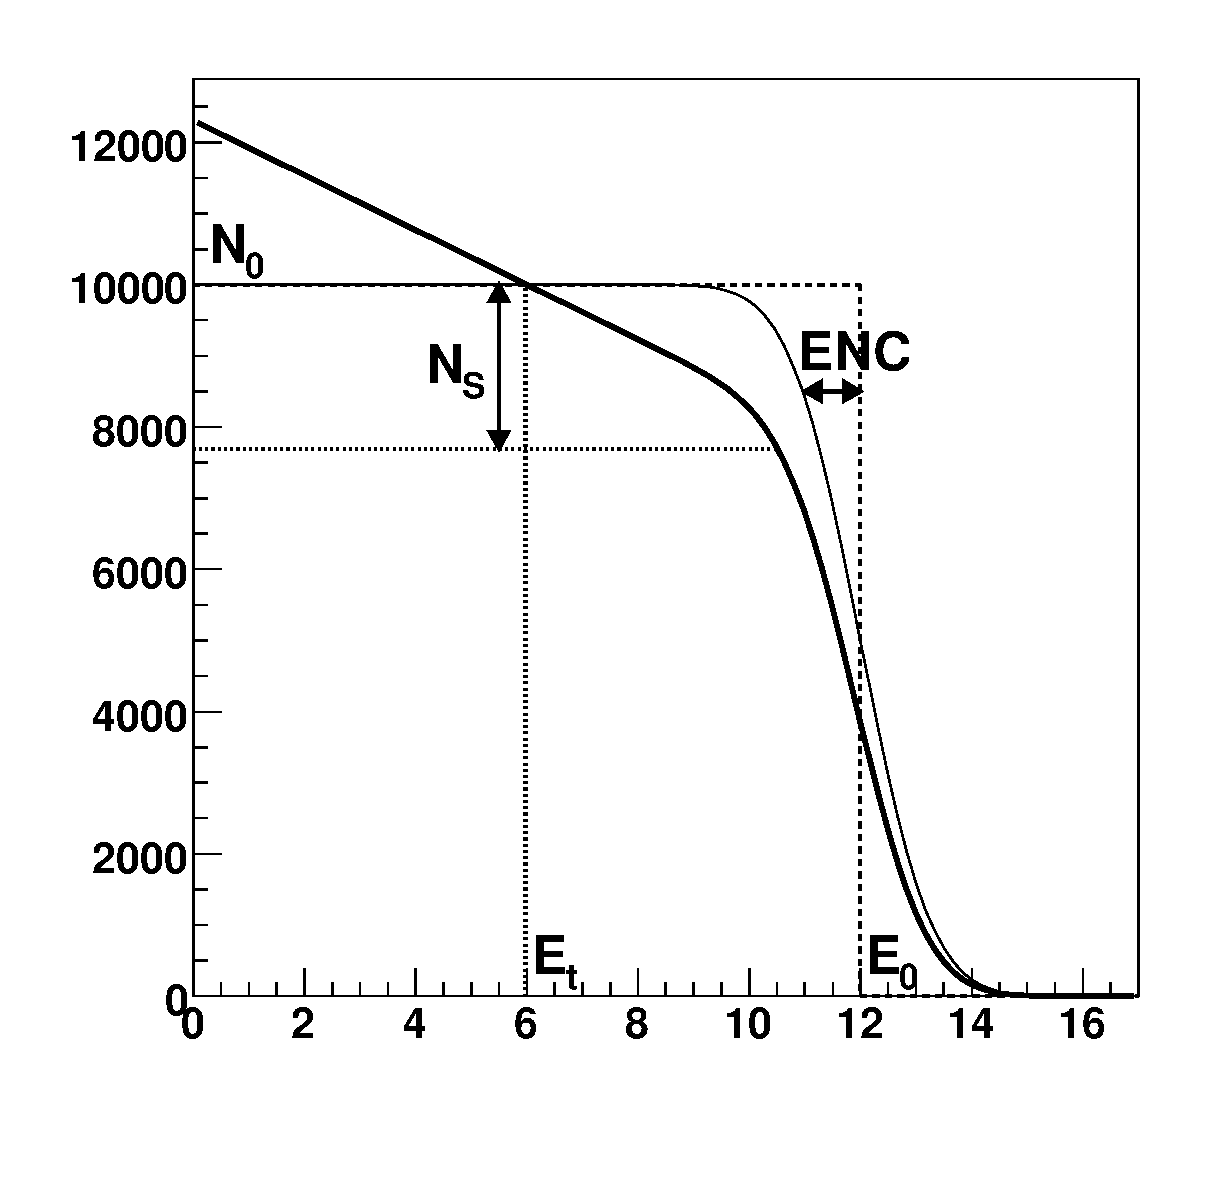
\includegraphics[width=\textwidth]{images/thr_scan_expl}
\end{center}
\caption{Number of counts as a function of the threshold detected in an ideal case.}\label{fig:thrscan}
\end{figure}

\begin{figure}[t!]
\begin{center}
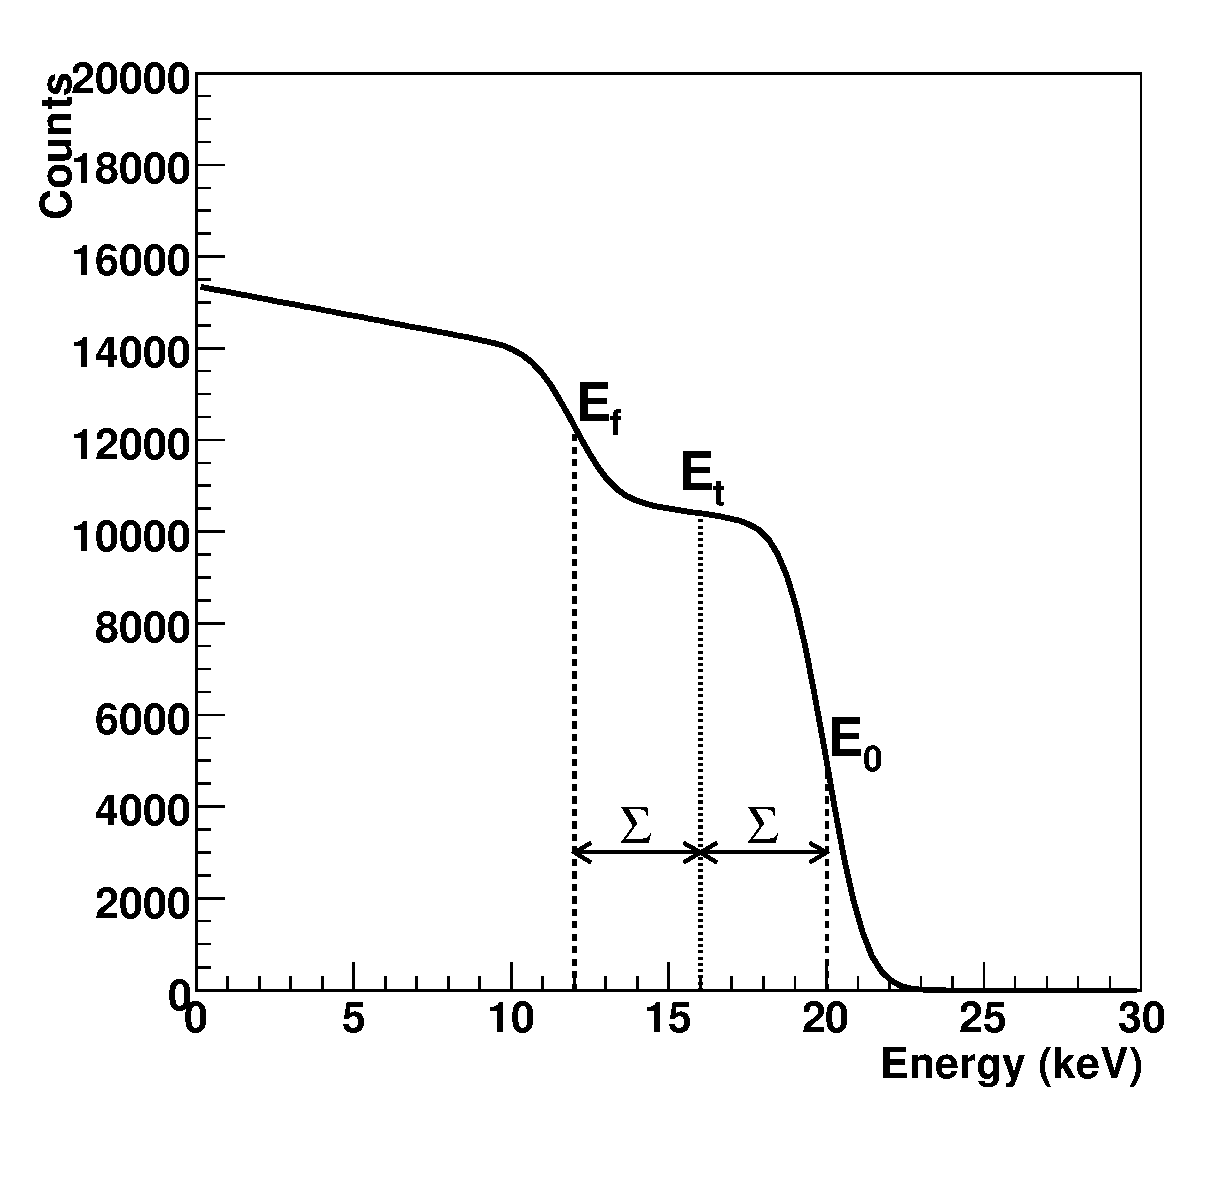
\includegraphics[width=\textwidth]{images/thr_scan_fluo}
\end{center}
\caption{Number of counts as a function of the threshold detected in presence of fluorescent radiation}\label{fig:thrscanfluo}
\end{figure}

Once selected the settings, the threshold should be selected.
Figure~\ref{fig:thrscan} shows the number of counts as a function of the threshold value in the ideal case of monoenergetix X-rays of energy $E_0$=10~keV.
For thresholds larger than the X-ray energy the detector should always count 0 and for lower thresholds it should always count all the photons. However the curve is smoothed around $E_0$ because of the electronic noise (ENC) and is not perfectly flat for lower energies because the photons absorbed in the region between two strips distribute their energy between them and it is not flully collected by a single channel (charge sharing).\\
In order to count once al X-rays the threshold should be set at half of the X-ray energy $E_t=E_0/2$: if the threshold would be higher some photons would not be counted, leading to a loss of efficiency, while if it would be lower some photons would be counted twice leading to a loss of spatial resolution. 

Since the detector threshold can't be precisely set at the same value for all channels but there will always be some spread of the order of 200~eV (threshold dispersion) there will always be some fluctuations on the number of counts between channels, which however should be corrected by the flat field correction.

The choice of the threshold should also depend from  considerations regarding the emission of fluorescent radiation from the sample.\\
Figure~\ref{fig:thrscanfluo} shows  how the curve of the counts would look like for monochromatic X-rays of energy $E_0$ in presence of radiation of energy $E_f$ emitted by the sample. The curve would show a second step at $E_f$. 

Since the fluorecence emission is not present in the flat field data, the difference of counts between the channels due to the fluorescent radiation cannot be corrected and the threshold $E_t$ should be set at an energy larger than $E_f$. This also helps to cut down the background.\\
The difference of counts between the channels will be particularly large if the threshold is set in some ``steep'' part of the curve i.e. close to $E_f$ or to $E_0$ (but in this case it would be corrected by the flat field, at cost of loss of efficiency).
Because of the presence of the electronic noise, $E_t$ should be at least 3~keV larger than $E_f$.

Here is a short list of rules to select the appropriate working threshold in order of importance (and eventually modify the X-ray energy):
\begin{enumerate}
\item List the fluorescent emission lines $E_f$ that you expect from your sample. 
\item If there is no fluorescent emission ($E_f<E_0$) $E_t=E_0/2$
\item If there is fluorescent emission 
\begin{enumerate}
\item $E_t>E_f+3$~keV
\item $E_t<E_0-3$~keV 
\end{enumerate}
If the range where both requirements are satisfied is large, try to increase the distance of $E_t$ from $E_f$ up to 5~keV and then set $E_t$ as close as possible to the ideal value $E_t=E_0/2$
\item If it is not possible to satisfy the previous minimal requirements:
\begin{enumerate}
\item If you need high quality data and you can sacrifice detector efficiency (a lot!)  $E_t>E_f+3$~keV
\item If you need fast measurments and you can sacrifice detector uniformity (difficult to say how much) and increase the background $E_t<E_f-3$~keV. Remember that $E_t$ is klimited by the electronic noise $E_t>4$~keV (3~keV for \textit{High gain} settings).
\item Consider to change $E_0$ to values lower than $E_f$ or at least 6-8~keV larger than $E_f$ 
\end{enumerate}
\end{enumerate}



\begin{figure}
\begin{center}
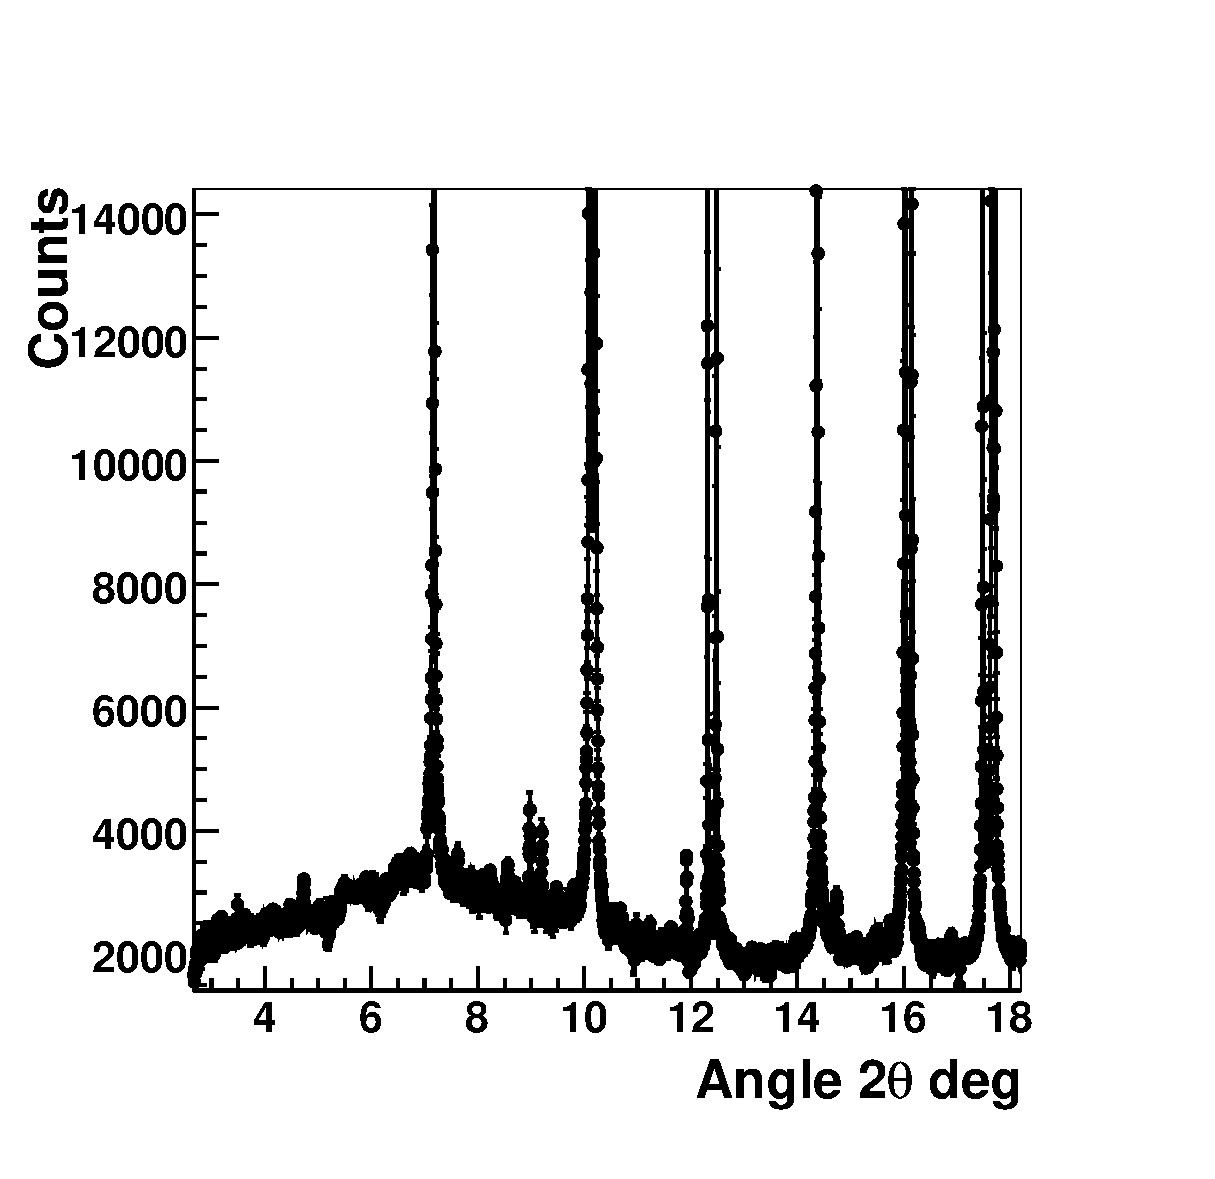
\includegraphics[width=\textwidth]{images/sample_with_fluorescence}
\end{center}
\caption{Example of data from a sample emitting fluorescent light and detector threshold set at a value close to the emission line. The background data cannot be properly flat field corrected.}\label{fig:samplefluo}
\end{figure}

\section{How does the flat field correction work?}



\subsection{Why isn't my flat-field flat?}

The main reasons of a non flat flat-field can be:
\begin{itemize}
\item The scattering from the glass rod is not uniform over the angular range. In this case you should take the flat field dynamically i.e. scanning the detector in front of the cylinder with the small window, as we do at the SLS. In this case when you shift the detector, the shape of the illumination remains in the same angular position (and shifts in channel number). Of course it depends a lot on the energy and on the geometry of the flat field acquisition.
\begin{figure}
\begin{center}
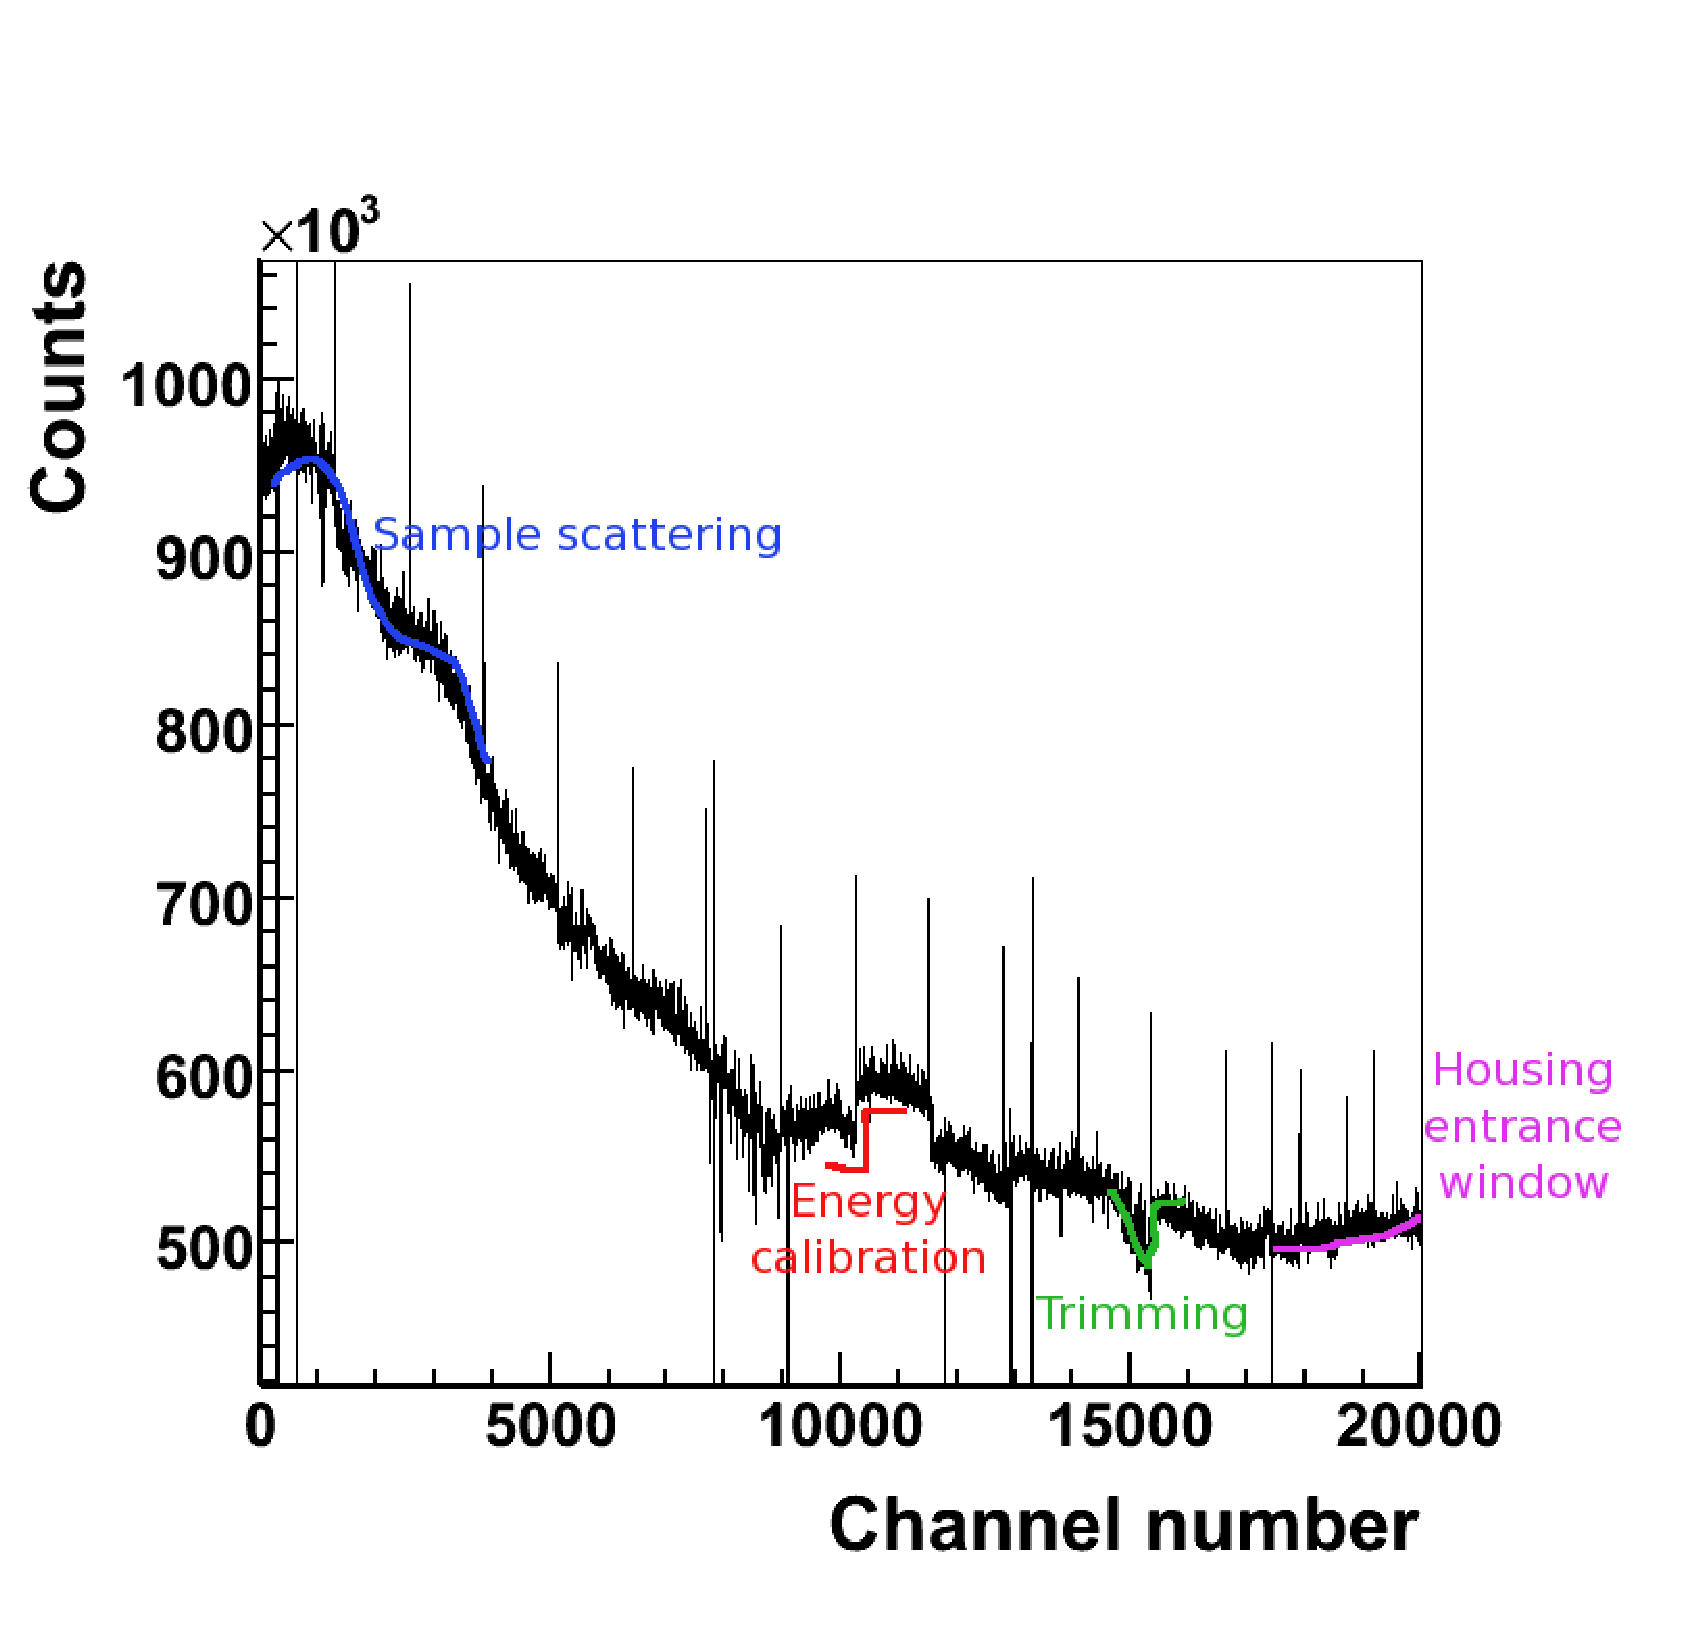
\includegraphics[width=\textwidth]{images/bad_ff_col}
\end{center}
\caption{Example of a very bad flat field data set with highlights of some of the reasons which can cause the non-flat behavior for the MYTHEN detector. Similar effects can be visible also in 2D.}\label{fig:badff}
\end{figure}

\item The entrance window for the X-rays is deformed (we also have this problem at the SLS). In this case when you move the detector the "mountain" moves with it in angle (And remains still in channel number). However this should correct without problems with the flat field correction, even in case of fluorescent emission. Should appear at all energies.
\begin{comment}
\begin{figure}
\begin{center}
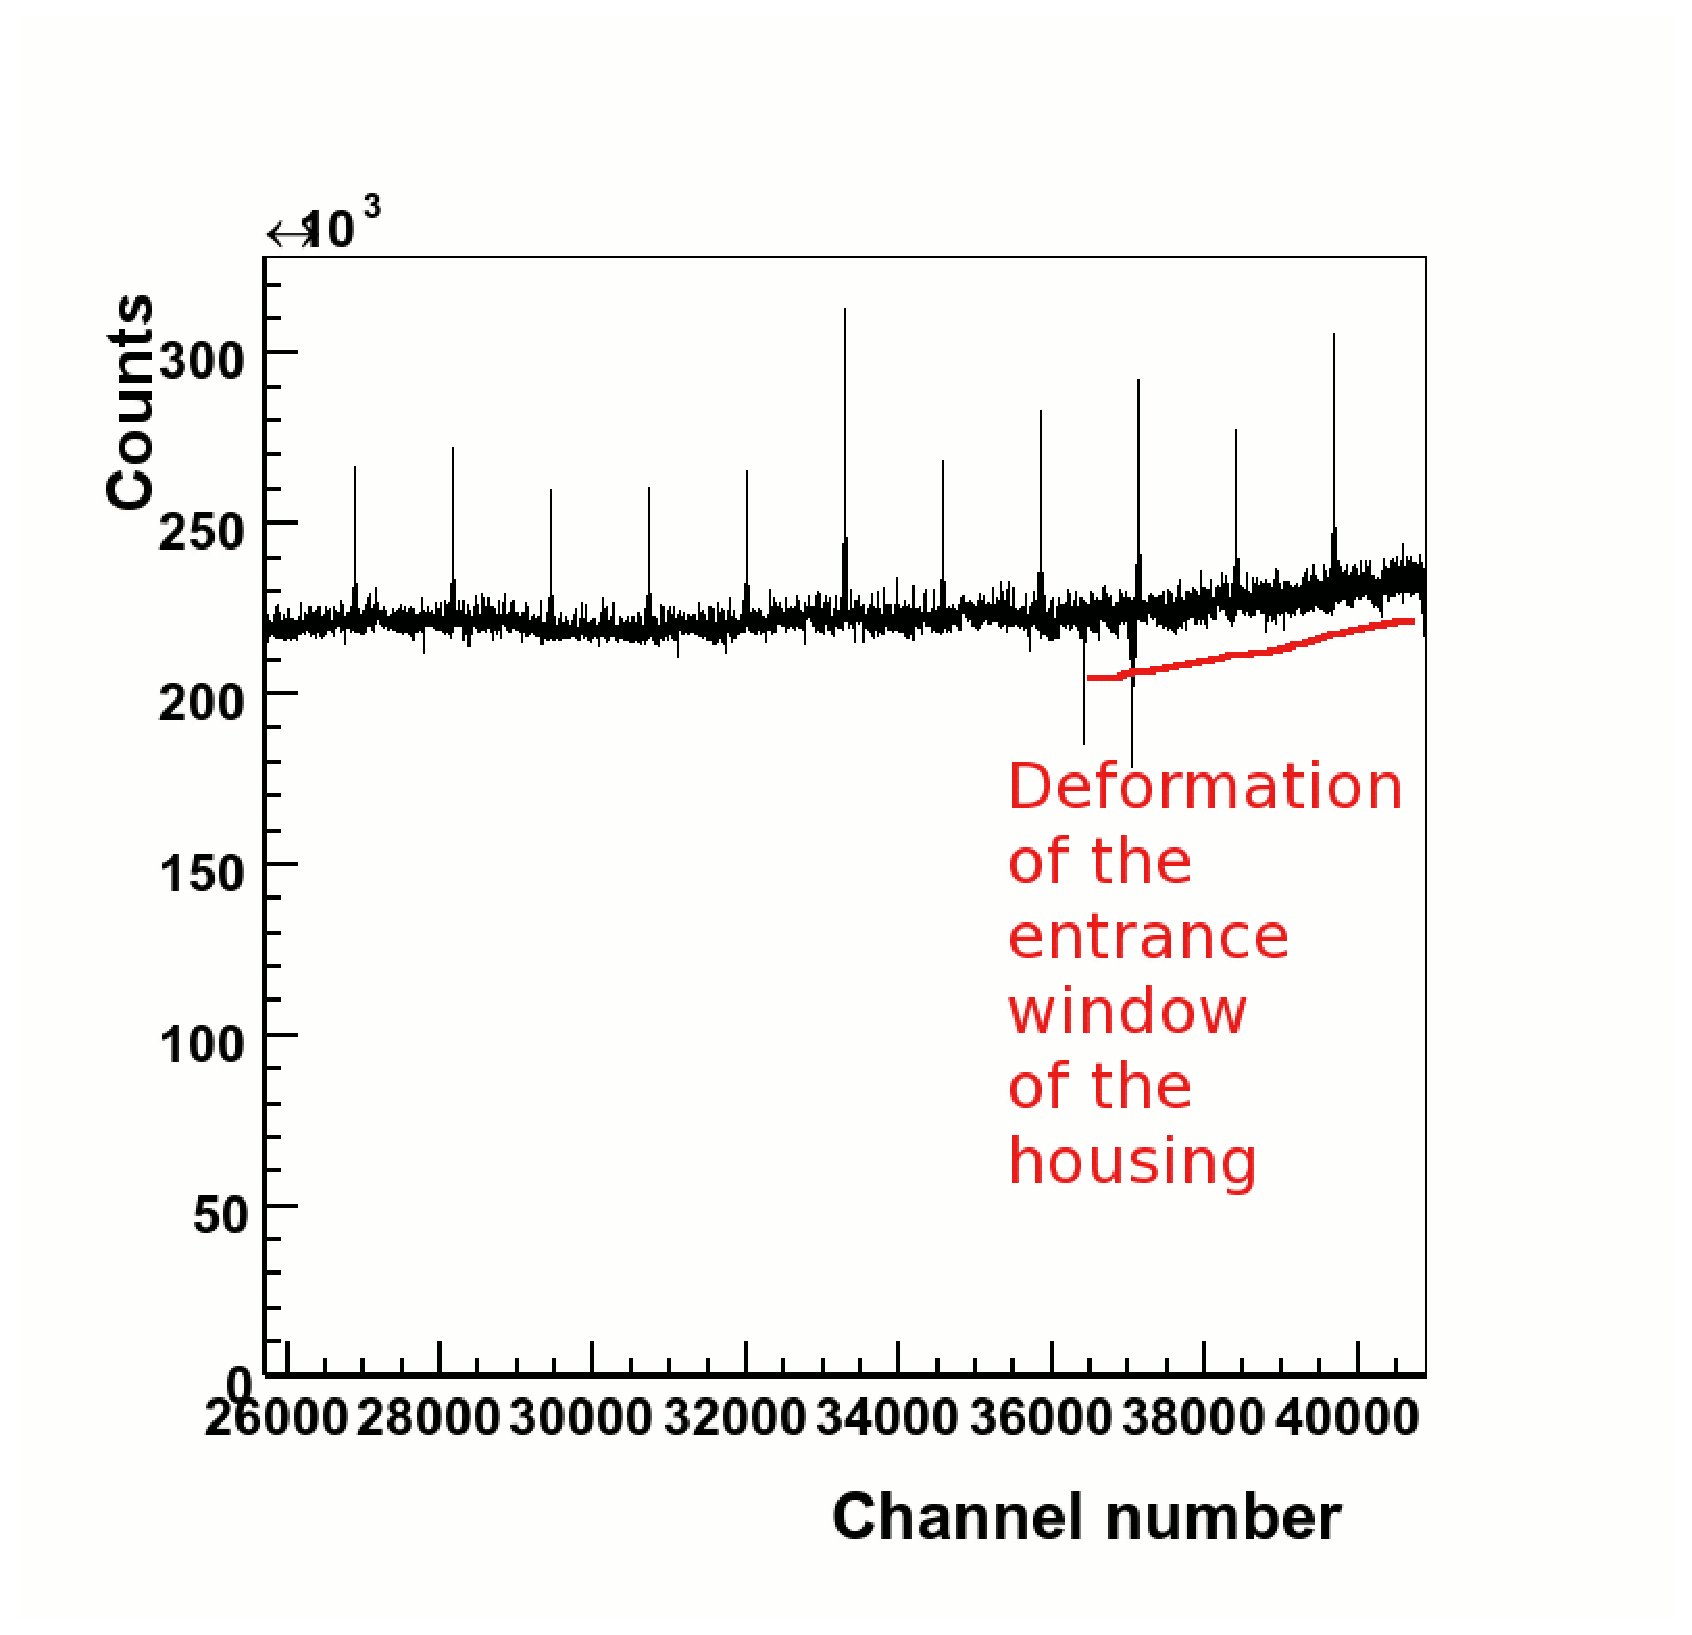
\includegraphics[width=\textwidth]{images/ff_window}
\end{center}
\caption{Variations in the flat field due to a non unifor entrance window of the detector housing.}\label{fig:ffwin}
\end{figure}
\end{comment}
\item Differences of efficiency between the modules i.e. mainly bad energy calibration. You normally see really steps at the transition between modules. Sometimes you have some groups of strips withing a module that are not properly trimmed and look as smallish peaks or valleys in the flat field. When you move the detector, these steps or peaks move in angle and remain still in channel number.
These differences can slightly change as a function of the energy (probably more evident at lower energies) but should normally always be there for the same settings.
These differences get much worse in presence of fluorescent emission, but normally correct properly with flat field correction.
\end{itemize}
\begin{comment}
\begin{figure}
\begin{center}
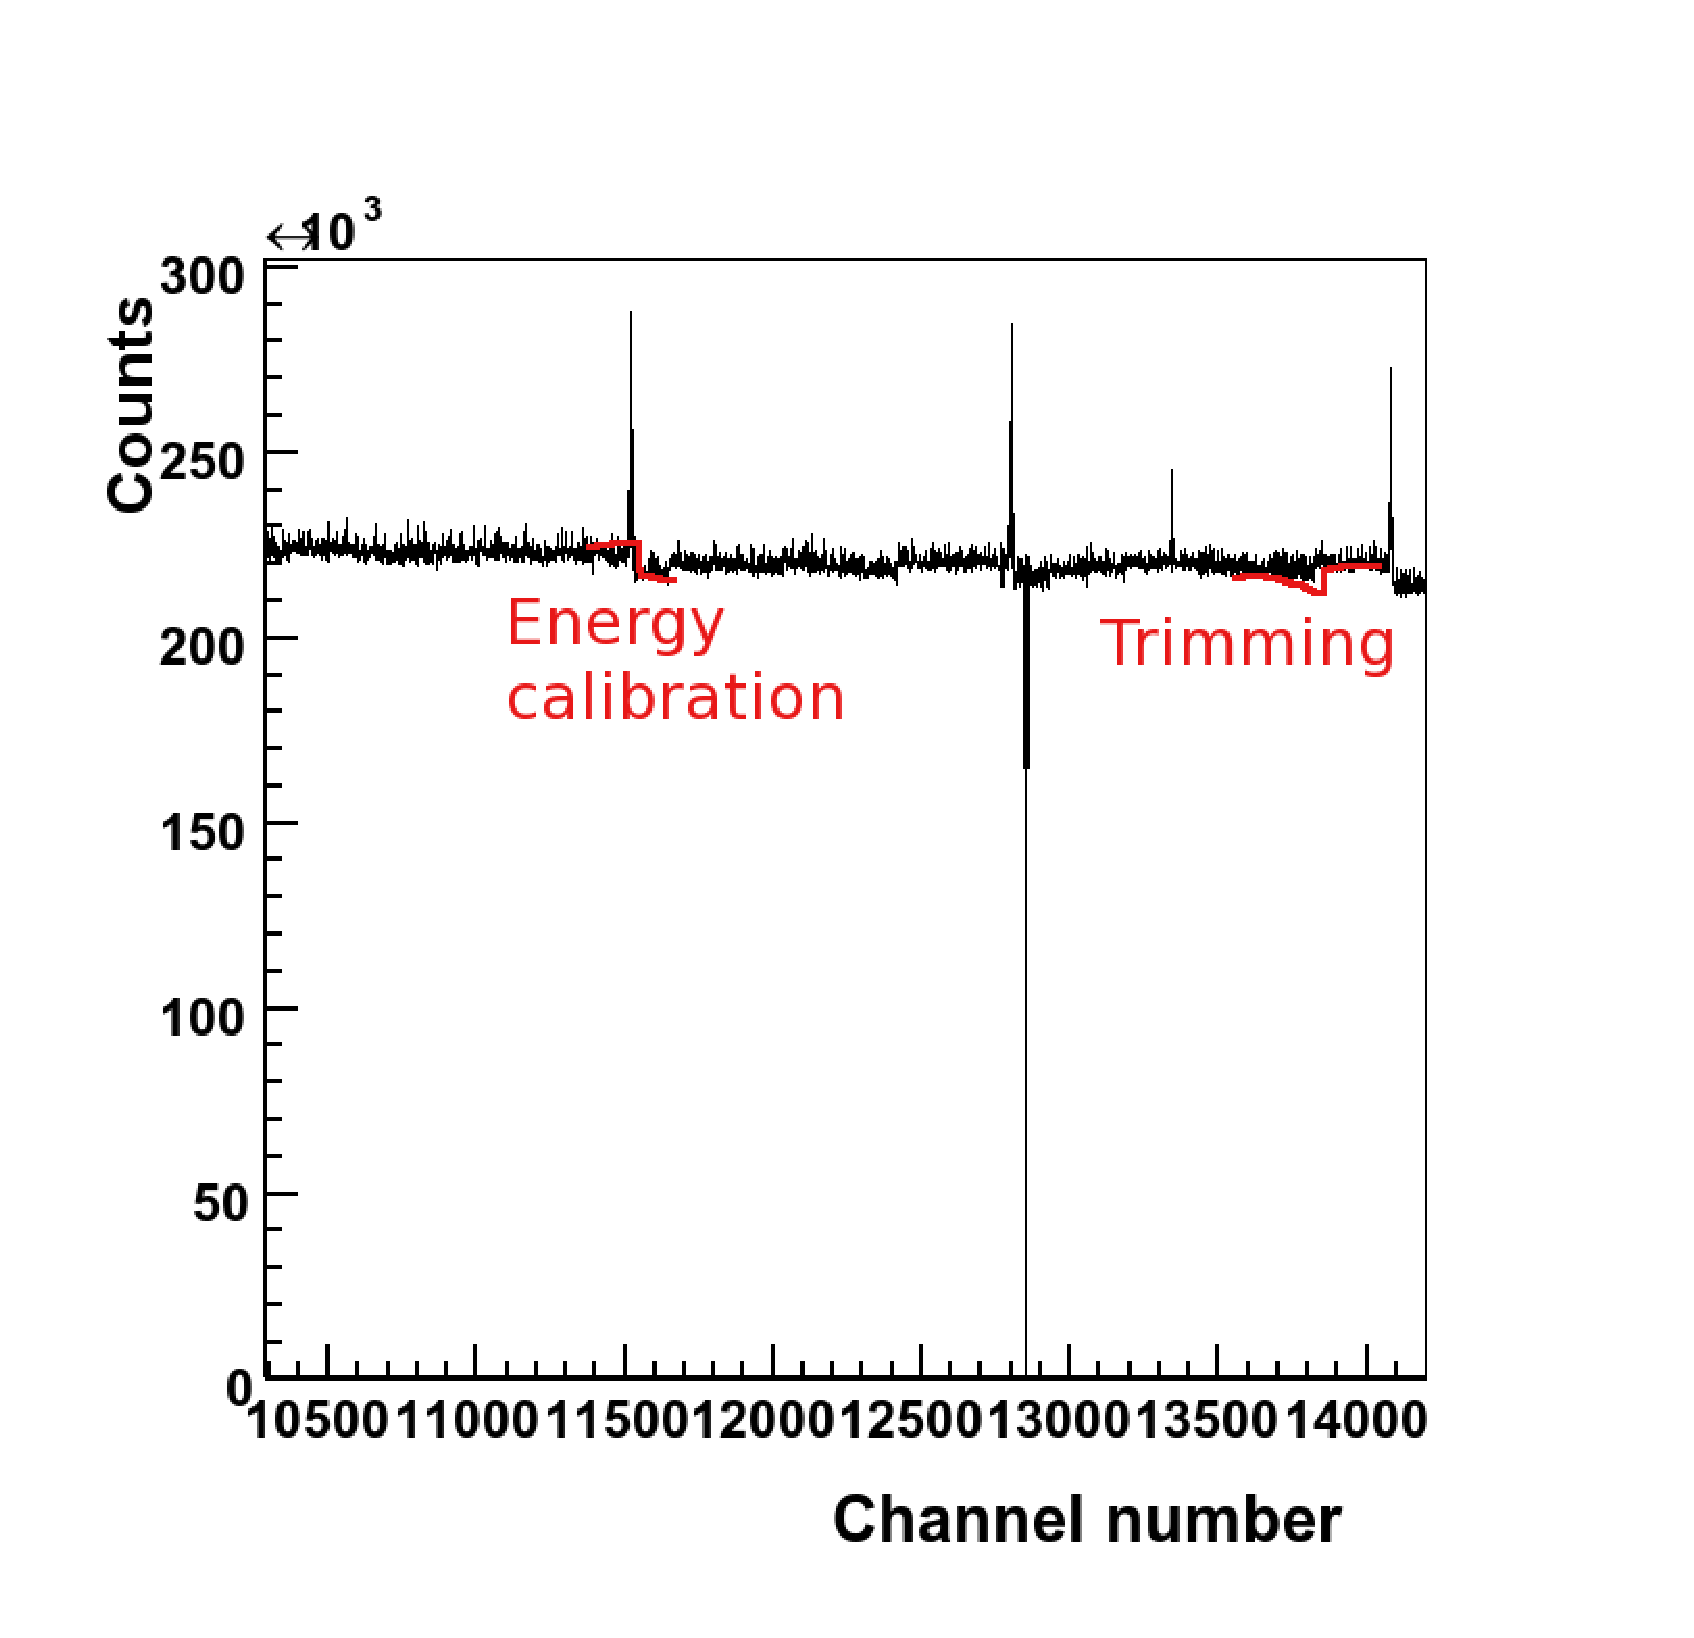
\includegraphics[width=\textwidth]{images/ff_calibration}
\end{center}
\caption{Variations in the flat field due to a non precise energy calibration or trimming of the detector modules for the MYTHEN detector. Similar effects can be visible also in 2D.}\label{fig:ffcal}
\end{figure}
\end{comment}

\subsection{Dynamic acquisition of the flat field}

In case it is not possible to uniformely illuminate the detector due to its large dimensions, one of the solutions is to scan it in front of an illuminated are with a uniform speed such that the integrated number of counts during the exposure time is the same for all channels.\\

To do that, at the SLS we have optimized the dynamic acquisition of the flat fiel with the MYTHEN detector using a setup similar to the one sketched in figure~\ref{fig:ffsetup}.
It is important that the scanning range of the detector is chose such that the detector is not illuminated both at the beginning and at the end of the acquisition. Moreover the movement of the detector should be as uniform as possible. To avoid this kind of systematic errors we normally sum two flat field images taken in the two opposite directions of translation.\\

Also take care that your sample does not emit fluorescent light at the chosen energy (e.g. a glass rod works at all energies, but heavier materials can be chosen to increase the efficiency at higher energies taking care that the fluorescence emission is negligible).

\begin{figure}
\begin{center}
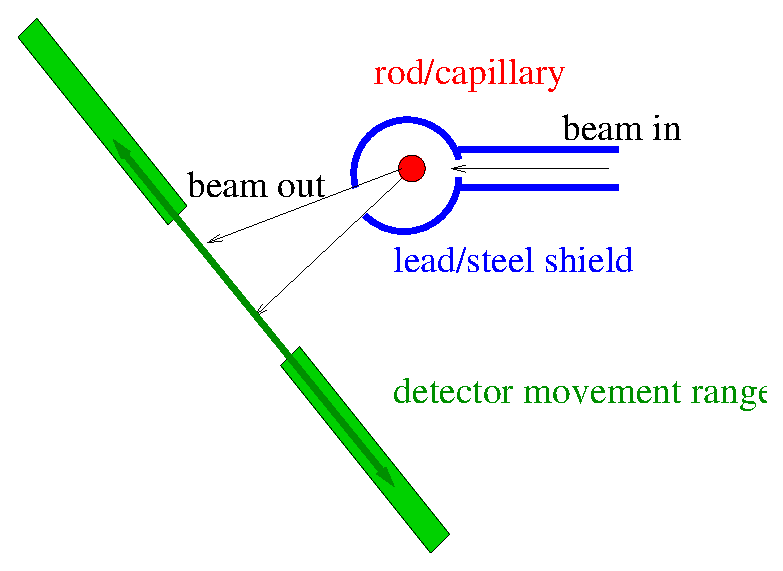
\includegraphics[width=\textwidth]{images/FFSetup}
\end{center}
\caption{Sketch of the experimental setup for a dynamic acquisition of the flat field.}\label{fig:ffsetup}
\end{figure}

\section{What happens when I trim the detector?}

General remarks about trimming.

\subsection{MYTHEN}

%\subsubsubsection{Trimming with noise} \label{sec:noisetrim}
\textbf{Trimming with noise} \label{sec:noisetrim}\\

The first step in the trimming procedure is to trim with noise (this is often sufficient). This has to be done for all the settings which are foreseen to be used (highgain, standard and fast).\\
The procedure for the noise trimming is as follows:
\begin{enumerate}
\item In the \textit{Initialization tab} click on the settings for which you want to trim (e.g. standard)
\item In the \textit{Initialization tab} click on the \textit{advanced} radio button to make the trimming accessible.
\item  In the \textit{Acquisition tab} set the acquisition time to 100~ms, the repetion to 1 and the delay between frames to 0.
\item For noise trimming usually the default parameters $Vthreshold=7$, $Counts=500$, $Resolution=4$ work.\\
However, to verify the threshold setting it is best to make a threshold scan. To do this go to the \textit{Data} tab, in the Data display section select the 2D color and type advanced option. In the \textit{Acquisition} tab select your data directory. Set the number of positions to 0. Select Scan, Type threshold. Typical values for the range are 500 to 900 with a step size of 10. Then click on the start button to perform the threshold scan. After the threhold scan has finished an image similar to the one in~\ref{fig:thresholdscanuntrimmed} should be shown. Depending on the system the number of modules may vary. If the plot is similar to the one in~\ref{fig:thresholdscantrimmed} the noise trim files did already exist and have been loaded when selecting the settings. In this case you don't need to trim with noise again.\\
Set the parameter Vthreshold in the \textit{Trimming} box (\textit{Initialization tab}) 10-30 DAC units below the onset of the noise for the module with the lowest threshold offset. Since the modules have differences in the offset and gain the onset of the noise varies. \\
You can usually leave the remaining parameters unchanged (Counts/pixel=500; Resolution=4).
\item Select the directory where the noise trim files should be written and the filename, to wich will be attached the extension given by the module serial number (.snxxx). If you want the trimfiles to be loaded authomatically when the global settings are selected, select the default directory specified in the config file (or in the ``trimbits/beamline'' directory for the older software versions). 
Click on \textit{Trim} to start the noise trimming process. After the trimming has finished look at the plot and the distribution of the trim bits. The distribution should be around 32$\pm$5 and should look gaussian. An example distribution is shown in figure~\ref{fig:trimdistribution} and an example plot in~\ref{fig:trimplot}. If the distribution is too much off center change the counts/pixel, if it is too narrow reduce the resolution (set it to 3), if it is too wide increase it (set it to 5). Make sure not too many channels have a trim value of 0 or 63.
\item Execute the treshold scan again to verify the trimming was done properly. A plot similar tho the one in figure~\ref{fig:thresholdscantrimmed} should appear.
\end{enumerate}

\begin{figure}
\begin{center}
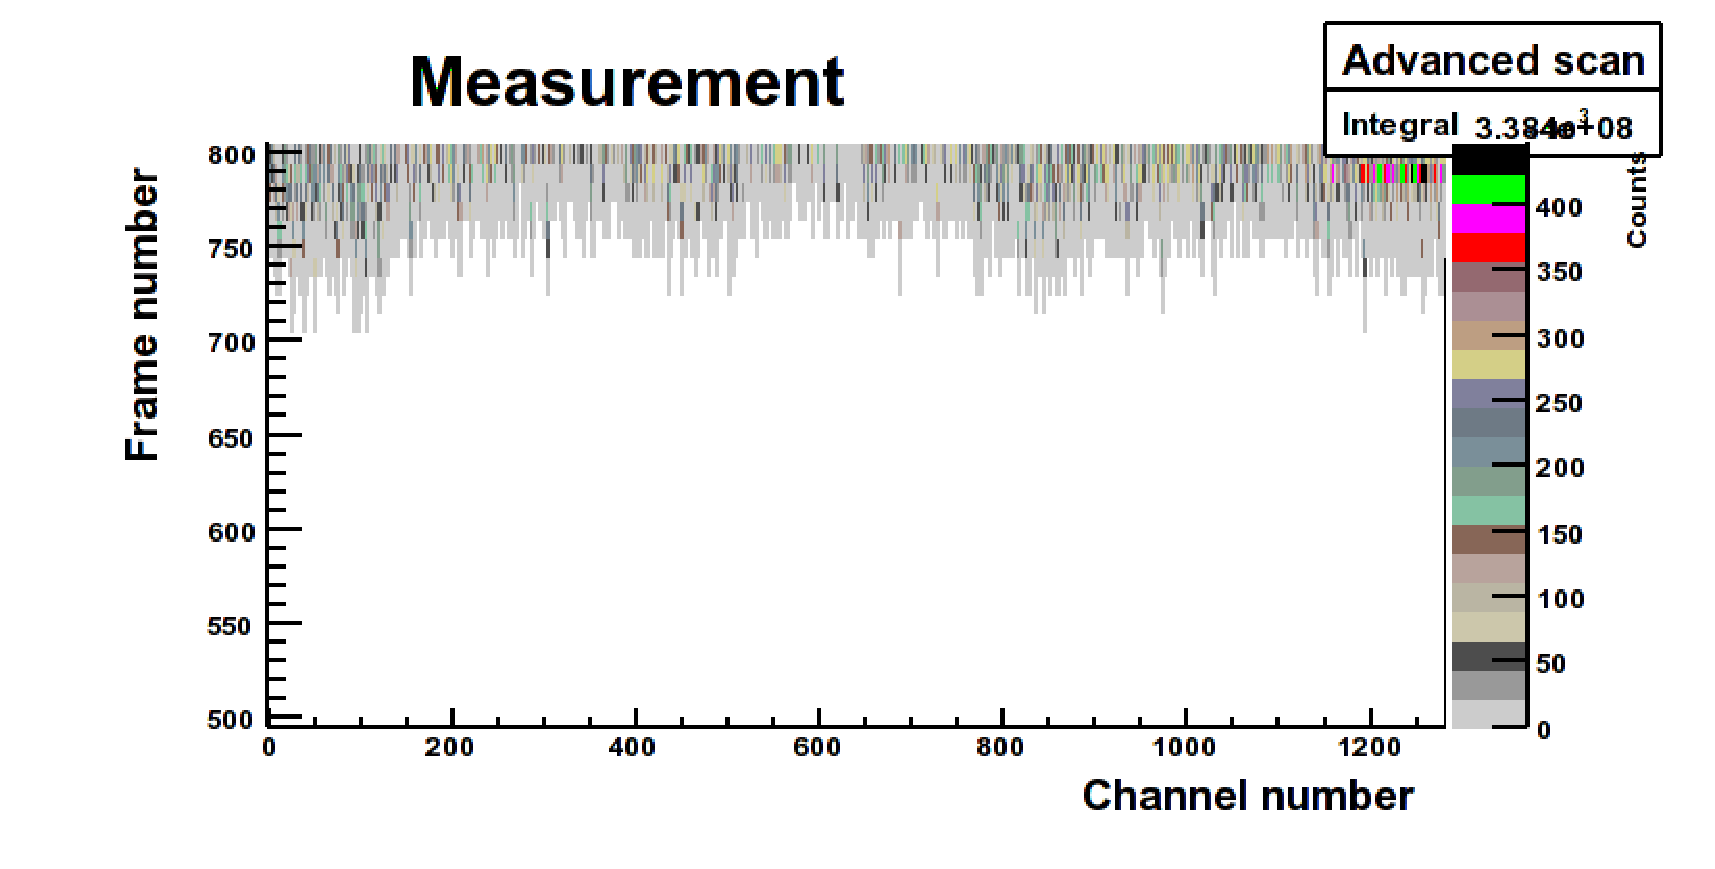
\includegraphics[width=\textwidth]{images/noise_thresholdscanuntrimmed}
\end{center}
\caption{The untrimmed threshold scan.}\label{fig:thresholdscanuntrimmed}
\end{figure}

\begin{figure}
\begin{center}
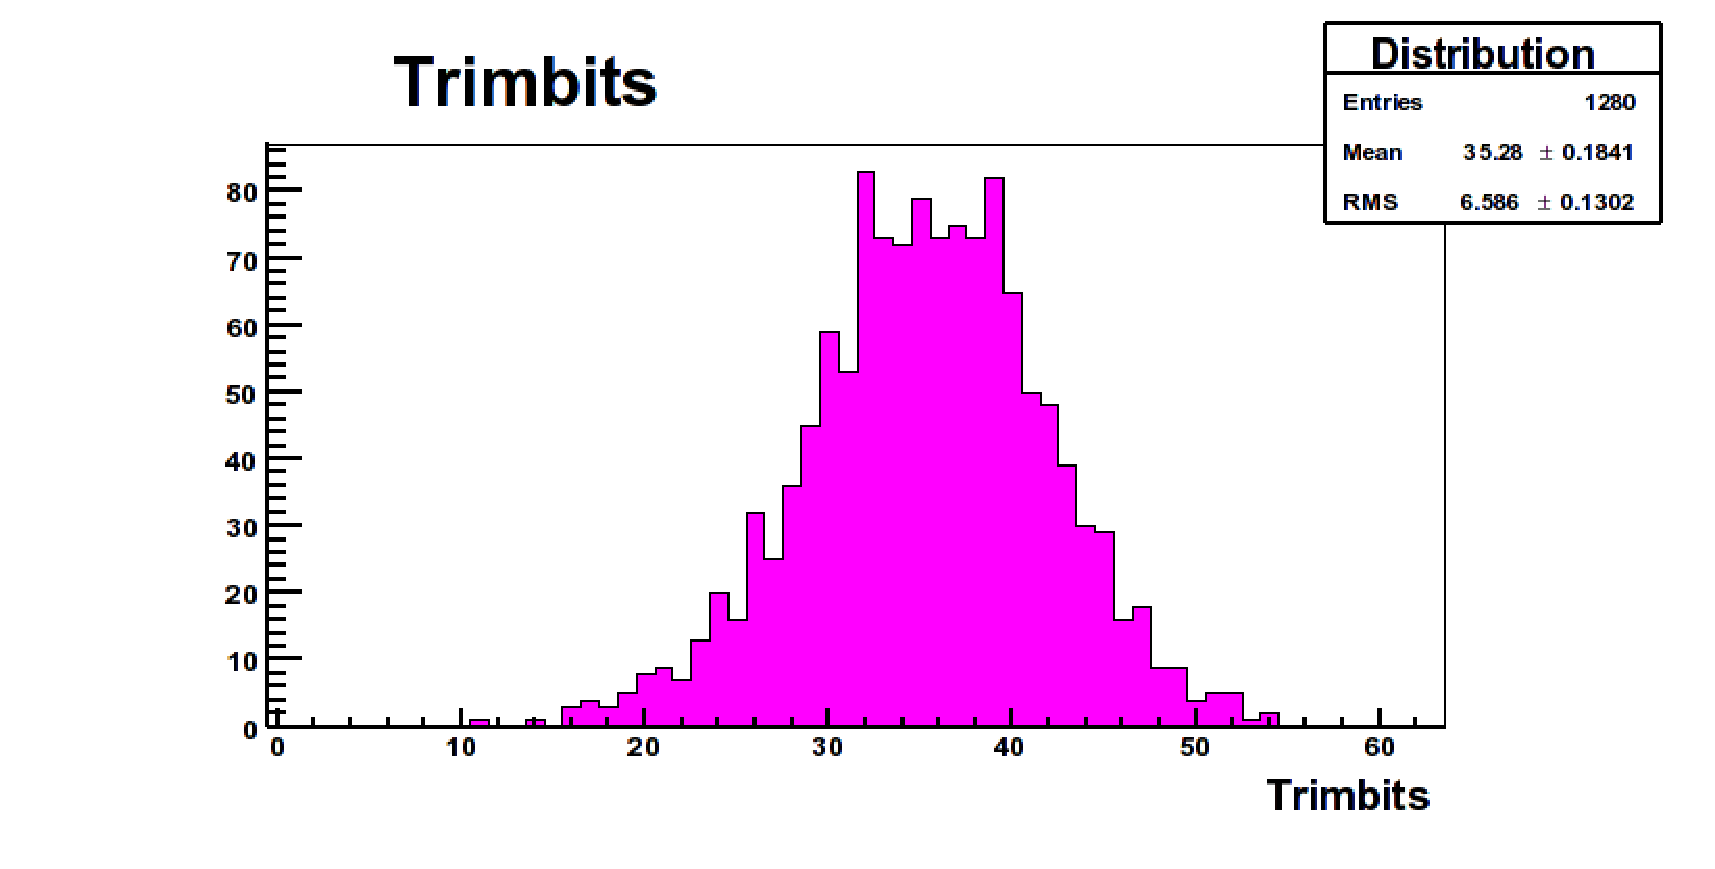
\includegraphics[width=\textwidth]{images/trimbitdistribution}
\end{center}
\caption{The distribution of the trimbits.}\label{fig:trimdistribution}
\end{figure}

\begin{figure}
\begin{center}
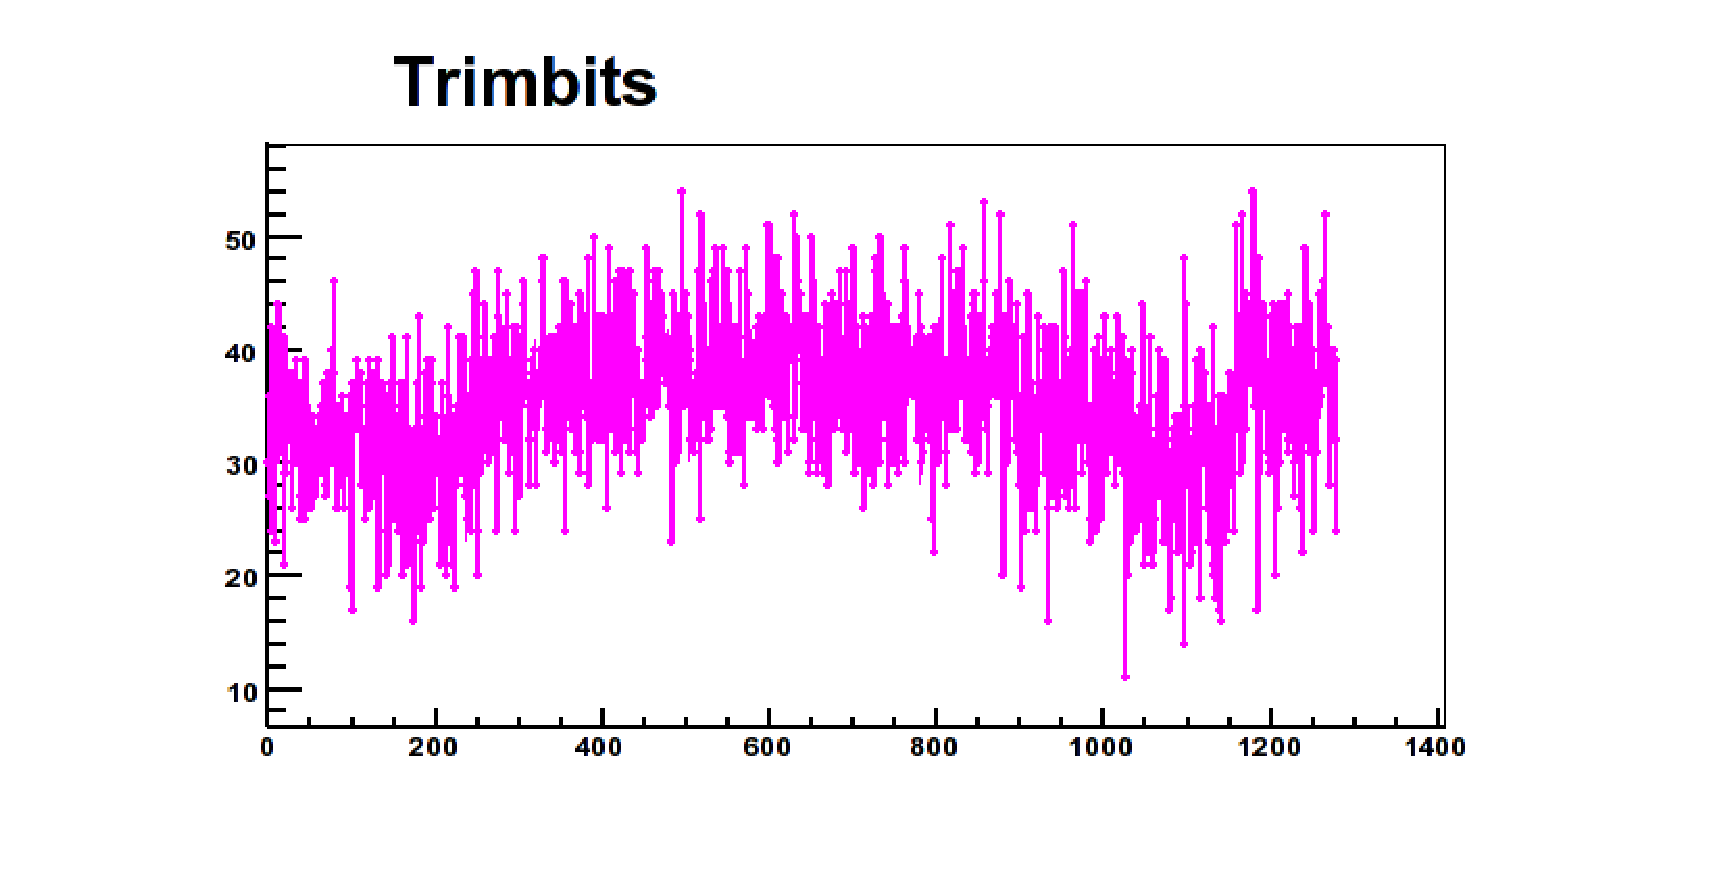
\includegraphics[width=\textwidth]{images/trimbitplot}
\end{center}
\caption{The trimbits for all the channels.}\label{fig:trimplot}
\end{figure}

\begin{figure}
\begin{center}
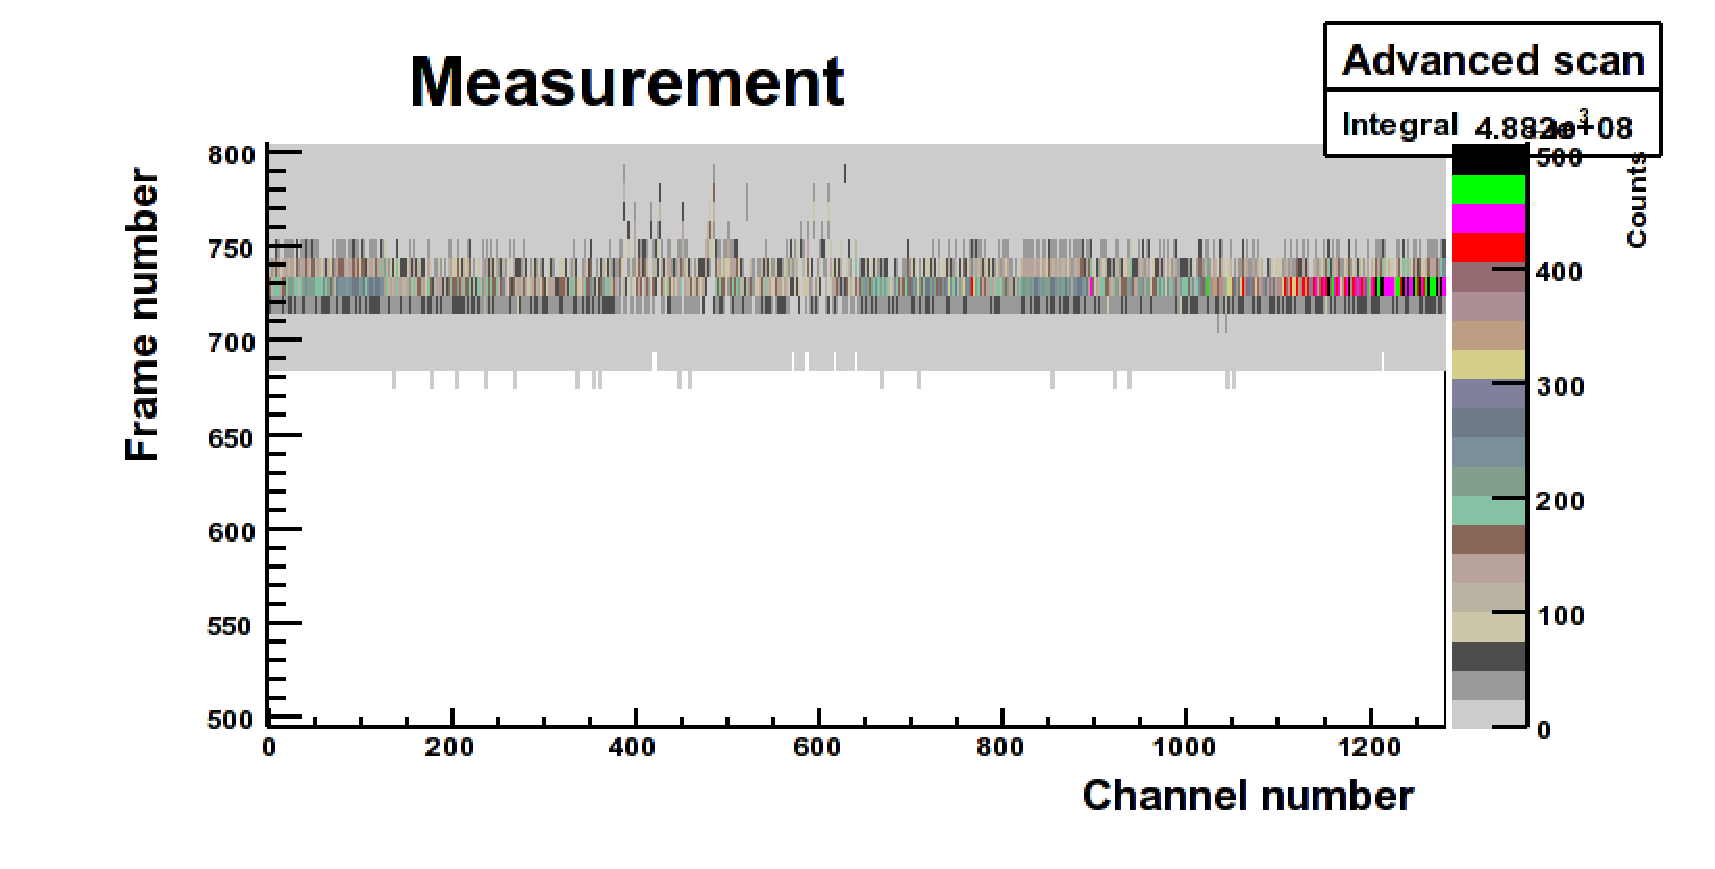
\includegraphics[width=\textwidth]{images/noise_thresholdscantrimmed}
\end{center}
\caption{The trimmed threshold scan.}\label{fig:thresholdscantrimmed}
\end{figure}



\textbf{Improve the trimming using X-rays}\label{sec:improvetrimming}\\

The improvement of the trimming acquired with noise is not essential: at 12~keV an untrimmed module has a threshold dispersion which is about 1.4~keV and is already reduced to 200~eV at 12~keV by the noise trimming. At lower energies the noise trimming will be more effective, while the threshold dispesion will be still larger at higher energies. The trimming improvement reduces the threshold dispersion to 140~eV at 12~keV and is expected to be almost constant at all energies. For this reason it is suggested to perform the trimming improvement only when a small threshold dispersion is really important (e.g. to avoid flat field corrections or in presence of fluorescent lines close to the threshold value) and it will probably be not worthy at lower energies (i.e. threshold lower than 6~keV and X-ray energy lower than 12~keV). 
The procedure for the trimming improvement is as follows:
\begin{enumerate}
\item Select the settings of the detector and load the noise trimming file
\item Set the threshold at half of the X-ray energy (better if the detector has already been calibrated in energy like explained in~\ref{sec:encal})
\item Illuminate the detector with a flat field. This is very important to obtain a good trimming. 
\item Select the \textit{acquisition time} in the \textit{acquisition tab} so that there are at least 1000 counts/strip per frame (the more counts, the better trimming). Set the repetions to 1 and the delay between frames to 0.
\item Go to expert mode by clicking on \textit{advanced} in the \textit{initialization tab}, \textit{settings} box
\item In the trimming box  select the directory where the noise trim files should be written and the filename, to wich will be attached the extension given by the module serial number (.snxxx).
\item Select the \textit{improve} method
\textit Start the trimming
\end{enumerate}
If the trimming is correctly performed and the illumination is flat enough, the same trimming can be used every time you will measure at this same energy.
The authomatic loading of energy-specific trim files is not yet implemented.

\section{In what consists the energy calibration of the detector?}\label{sec:encal}

General remarks about DAC to energy conversion

\subsection{MYTHEN}

Since the conversion between the threshold DAC units and energy depends on the gain and offset of the channels the energy calibration has to be done for all settings (high gain, standard and fast). For each setting follow this procedure:
\begin{itemize}
\item Select the setting in the \textit{Initialization} tab.
\item Enter in expert mode by clicking the \textit{Advanced} radiobutton in the \textit{Global settings} box in the \textit{Initialization} tab.
\item If the trimfiles are in the correct location and with the correct name, they should be loaded by default every time you select the corresponding settings in the \textit{global settings} box in the \textit{initialization} tab~\footnote{The default name of the calibrated trimfiles is \textsf{trimbits/beamline/}\textit{settings}\textsf{/noise.snxxx} where  \textit{settings} is the chosen settings. You  can change it in \textsf{src/qDetector.h} and then recompile the acquisition program as described in~\ref{sec:installation}.}.
If the trim files do not yet exist generate them as explained in section~\ref{sec:noisetrim}.
\item Execute a threshold scan of the detector with at least three different energies. The more monochromatic are the X-rays, the better the calibration will be (i.e. scattered X-rays are better than the fluorescent emission). \\
The scan should range from where all modules count 0 (estimate 850-20$\cdot$energy(keV) DAcu) and where all modules start having a lot of noise (usually 800 DACu) with a step of 1 or 2 DACu. The acquisition time should be chosen so that there are at least 1000 counts per strip on the plateau.
\item Open the file \textsf{root/CalAllModules.C} for editing. Change the value of the following global variables according to your needs:
\begin{itemize}
\item \textit{nmod} is the number of modules of your system.
\item \textit{nscan} is the number of different threshold scans you acquired.
\item \textit{en} is the array with the energies at which you acquired the scans, in keV.
\item \textit{een} is the array with the errors on the energies at which you acquired the scans, in keV. It is usually small, but can be some hundreds eV in case of dirty fluorescent samples.
\item \textit{fn} is the array containing the location and root file name of your data.
\item \textit{run} is the array containing the run index of your data.
\item \textit{startscan} is the array containing the threshold value at which you started the scans.
\item \textit{stopscan} is the array containing the threshold value at which you finished the scans.
\item \textit{stepscan} is the array containing the threshold step of the scans.
\item \textit{ave} is the array containing the average number of counts per strip on the plateau (it must not be too precise).
\item \textit{sn} is the array containing the list of the serial number of the modules to be calibrated. It is important that the list is in the right order, so that the optput calibration files have the extension .snxxx corresponding to the right module.
\item \textit{of} is the location and root file name of the calibration file. The directory should already exist and the extension .snxxx will be attached to the output file.  
\end{itemize}
\item Launch \textsf{root}, which you should have already installed on your linux PC
\item Execute the following commands in order to load the macros needed for the calibration:
\begin{verbatim}
root$ .L root/NewMythenMacros.C++
root$ .L root/CalAllModules.C++
\end{verbatim}
You should get a lot of warnings, but no errors.
\item Execute the following command in order to run the calibration:
\begin{verbatim}
root$ EnCalModules()
root$
\end{verbatim}
Reading and analyzing the data takes some time, but, after a while, a canvas should open where the plots of the median of the counts of every module as a function of the threshold should be shown for each energy, fitted with a modified \textit{erf} function in order to find the inflextion point. The last plot of the canvas should represent the inflexion points as a function of the energies, and by fitting it with a straight line it is possible to calculate the offset and gain for each module i.e. calibrate it as a function of the energy. Please check that this automated fitting procedure succeeds. In case you see many fitting errors you should try to check wether the variable you edited in  \textsf{root/CalAllModules.C} are all correct or try to edit the fitting procedures in the two root macro files (sorry!).
\item Copy the calibration file you obtained to \textsf{calibration}/\textit{settings}\textsf{.snxxx}~\footnote{The default name of the calibration file \textsf{calibration/}\textit{settings}\textsf{.snxxx} where  \textit{settings} is the chosen settings. You  can change it in \textsf{src/qDetector.h} and then recompile the acquisition program.} By doing this the correct threshold for each module will be calculated every time you change the \textit{threhsold energy} in the \textit{global settings} box in the \textit{initialization} tab, you have loaded some default settings and you are not in expert mode.  
\end{itemize}

\section{Why should I change the dynamic range of the counters?}

\section{When should I enable rate correction}
\subsection{How can I choose the dead time?}

